React (иногда React.js или ReactJS) — JavaScript-фреймворк с открытым исходным кодом для разработки пользовательских интерфейсов.
React разрабатывается и поддерживается Facebook, Instagram и сообществом отдельных разработчиков и корпораций.React может использоваться для 
азработки одностраничных и мобильных приложений. Его цель — предоставить высокую скорость, простоту и масштабируемость. В качестве библиотеки для разработки 
пользовательских интерфейсов, React часто используется с другими библиотеками, такими как Redux.
Сравнивать ReactJs с Angular или другими MVC фреймворками не имеет смысла, так как ReactJs – это только представление. React – это язык шаблонов в сочетании 
несколькими функциями, которые позволяют отрисовать HTML, т.е. результат работы React – это HTML. ReactJs реализует концепции реактивного программирования: изменение 
результата работы зависит от состояния компонентов. Так, A = B + C, и результат A всегда будет зависеть от значений B и C. ReactJs постоянно работает с DOM, перерисовывая 
его при изменении условий (та часть DOM, которую меняет ReactJs, называется компонентом). 
React разработан вокруг концепции многоразовых компонентов. Вы определяете небольшие компоненты, и объединяете их, чтобы сформировать более крупные компоненты.
Все компоненты, маленькие или большие, могут использоваться повторно, даже в разных проектах.

\subsubsection{Обоснование выбора библиотеки React}
Поскольку пользовательский интерфейс пользователя является полностью компонентной структурой\cite{genesisgui}, для ее реализации более естественно подходят компонентные фреймворки, позволяющие
реализовать дерево зависимостей, направленное сверху вниз (от больших уровней абстрации к более низким). Такая архитектура системы пользовательского интерфейса позволяет добиться лучшей расширяемости
и избежать гонок за право манипулации состоянием системы ввиду использования подхода <<Единого источника истины>> (Single source of truth). Компонентный пользовательский интерфейс также реализуется
в таких фреймворках, как vue.js и angular, однако в качестве основного был выбран React ввиду его первичности на рынке средств разработки GUI и развитого набора средств работы с парадигмой Redux.

\subsubsection{Создание компонента Button}

\begin{lstlisting}[language=TypeScript, label=lst:domain:typescript]
function Button (props) {

 return <button type="submit">{props.label}</button>;

}

ReactDOM.render(<Button label="Save" />, mountNode)
\end{lstlisting}

Важной особенностью ReactJs является использование JSX. Это надстройка на JS, позволяющая использовать про-XML синтаксис в 
Javascript коде. JSX – это сочетание javascript и html, которые в связке являются непривычным синтаксисом для большинства разработчиков. 
Стандартом считается разделение JS части от разметки, что усложняет слежение за изменениями HTML -> JS -> HTML. JSX позволяет видеть все процессы 
в одном месте, не отвлекаясь на сложности грамотного и валидного кода. После компиляции JSX получается чистый JS.

\begin{lstlisting}[language=TypeScript, label=lst:domain:typescript]
const InputForm = React.createElement(
 "form",
 { target: "_blank", action: "https://google.com/search" },
 React.createElement("div", null, "Enter input and click Search"),
 React.createElement("input", { className: "big-input" }),
 React.createElement(Button, { label: "Search" })
);
function Button (props) {
 return React.createElement(
   "button",
   { type: "submit" },
   props.label
 );
}
ReactDOM.render(InputForm, mountNode);
\end{lstlisting}

JSX запись соответсвующего компонента по своему внешнему виду напоминает HTML, встроенный в JavaScript, однако существует ряд ограничений на их определение.
Например, RSX ReactDOM компоненты не могут быть определены как список XML элементов -- обязательно наличие корневого XML элемента, оборачивающего все дочерние элементы.
В случае, когда необходимо вернуть из функции или передать в рендер-функцию набор элементов, они передаются в виде JavaScript Array, где у каждого элемента обязательно должно
быть установлено свойство <<key>>, необходимое для инкрементальной реиндексации дерева элементов. Свойство key должно быть уникально в рамках коллекции, поэтому его, как правило,
привязывают к случайному guid элементу, либо к хэш сумме неизменяемых элементов отображаемого компонента. Такой подход позволят эффективно перерисовывать дерево элементов
и отслеживать появление в дереве компонентов новых листьев.

\begin{lstlisting}[language=TypeScript, label=lst:domain:typescript]
const InputForm =
 <form target="_blank" action="https://google.com/search">
   <div>Enter input and click Search</div>
   <input className="big-input" name="q" />
   <Button label="Search" />
 </form>;

function Button (props) {
 return <button type="submit">{props.label}</button>;
}
ReactDOM.render(InputForm, mountNode);

\end{lstlisting}

\subsubsection{Преимущества использования React}

Использование изоморфного подхода помогает производить рендеринг страниц быстрее, тем самым позволяя пользователям чувствовать 
себя более комфортно во время работы с приложением. Поисковые системы индексируют такие страницы лучше. Поскольку один и тот же код может 
быть использован как в клиентской, так и в серверной части приложения, нет необходимости в дублировании одного и того же функционала. В результате время 
разработки и затраты снижаются
Virtual DOM может повысить производительность высоконагруженных приложений, что может снизить вероятность возникновения возможных неудобств и улучшает 
пользовательский опыт. Благодаря переиспользованию кода стало гораздо проще создавать мобильные приложения. Код, который был написан во время создания сайта, 
может быть снова использован для создания мобильного приложения. 

\subsubsection{Изоморфные приложения}

Изоморфные приложения или изоморфный JavaScript, это использование одно и того же кода как в серверной, так и в клиентской части приложения. При открытии 
сайта в браузере, содержимое страницы должно быть загружено с сервера. В случае с SPA-приложениями (Single Page Application), это занимает некоторое время. Во время загрузки 
пользователи видят либо пустую страницу, либо анимацию загрузки. 

\begin{figure}[ht]
\centering
  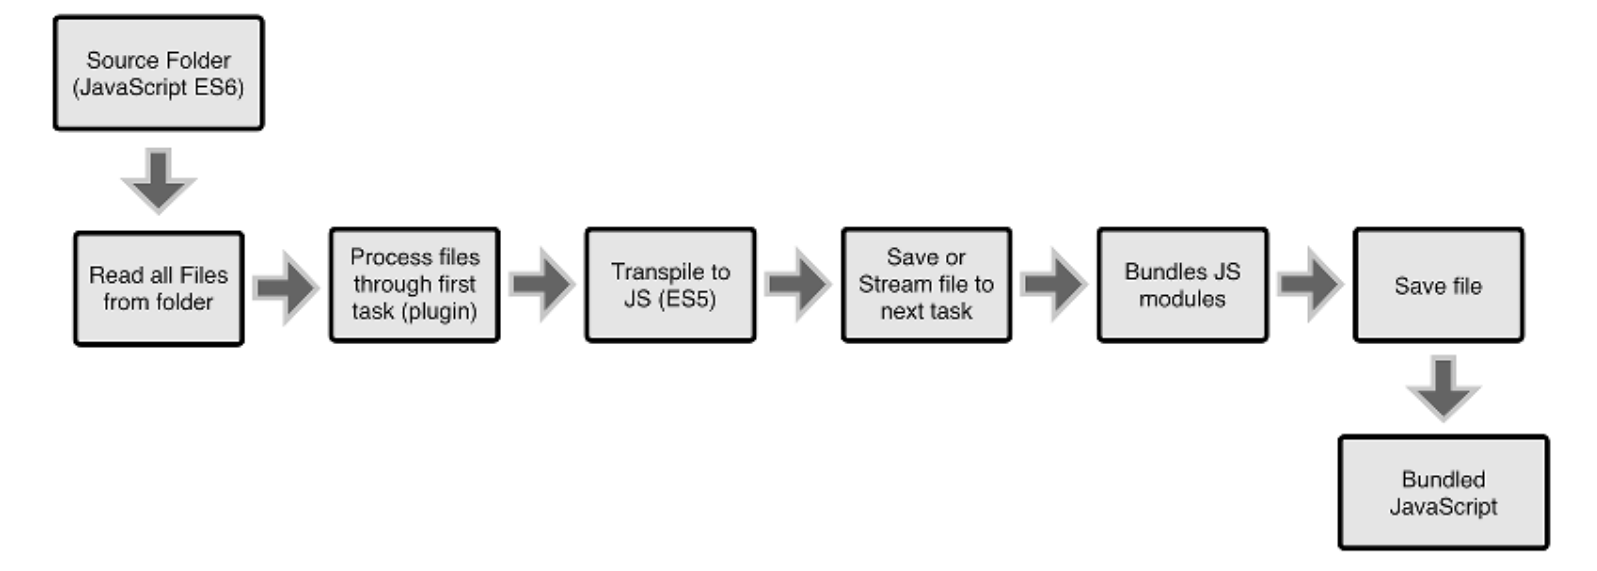
\includegraphics[scale=0.30]{react.png}
  \caption{Процесс загрузки изоморфных приложений}
  \label{figure:domain:react}
\end{figure}

Учитывая, что по современным стандартам ожидание в течение более чем двух секунд может быть весьма заметным неудобством для пользователя, сокращение времени загрузки 
является крайне важным преимуществом. Еще одна весомая проблема: поисковые машины плохо индексируют SPA-приложения. Исполнение JavaScript кода на стороне сервера исправляет 
подобную проблему. В случае с изоморфным приложением после загрузки страницы будет продолжаться рендеринг компонентов. Такая возможность рендеринга страниц как на сервере, так и 
на клиенте приводит к заметным преимуществам, таким как возможность лучшего индексирования страниц поисковыми машинами и улучшение пользовательского опыта. Более того, такой подход 
позволяет снизить время, затрачиваемое на разработку. При использовании некоторых современных фреймворков, вы должны создавать компоненты, которые должны рендериться на стороне сервера, 
а также шаблоны для клиентской стороны приложения. С помощью React можно создавать компоненты, которые работают на обеих сторонах.

\subsubsection{Document Object Model}

Document Object Model, или DOM, — это способ представления и взаимодействия с объектами в HTML, XHTML и XML документах. Согласно этой модели, каждый такой документ
представляет собой иерархическое дерево элементов, называемое DOM-деревом. Используя специальные методы, можно получить доступ к определенным элементам документа и 
изменять их в зависимости от нужных требований. При создании динамичной интерактивной веб-страницы необходимо, чтобы DOM обновлялся так быстро, как это возможно после 
изменения состояния определенного элемента. Для данной задачи некоторые фреймворки используют прием, который называется «dirty checking» и заключается в регулярном опросе 
состояния документа и проверке изменений в структуре данных. Подобная задача может стать самой настоящей проблемой в случае высоконагруженных приложений. Virtual DOM, в свою 
очередь, хранится в памяти. Именно поэтому в момент, когда «настоящий» DOM меняется, React может изменять Virtual DOM в мгновение ока. React «собирает» такие изменения сравнивает 
их с состоянием DOM, а затем перерисовывает изменившиеся компоненты.

При данном подходе не производится регулярное обновление DOM. Именно поэтому может быть достигнута более высокая производительность React приложений. Второе следствие вытекает 
из изоморфной природы React: можно производить рендеринг на стороне сервера совсем как на стороне клиента.

Для создания UI-интерфейса создается структура файлов и папок

\begin{lstlisting}[language=bash, label=lst:domain:typescript]
+-- js 
|   +-- react 
|       +-- react-dom.js 
|       +-- react.js 
|   +-- app.js 
+-- index.html 
+-- package.json 
+-- server.js
\end{lstlisting}

Babel — это компилятор, который транслирует любой диалект JavaScript, включая CoffeeScript, TypeScript и другие надстройки над языком в 
JavaScript ES5, который поддерживается почти всеми браузерами, включая IE8, если добавить babel-polyfill. Сила Babel в его модульности и расширяемости 
за счет плагинов. Например, уже сейчас можно использовать самые последние изменения JavaScript, не переживая, что они не будут работать в старых браузерах.
Для трансляции компонентов React в проекте можно использовать пресет babel-preset-react. Чтобы наш код корректно работал в старых браузерах, необходима установка 
пакета babel-polyfill, а babel-preset-es2015 и babel-preset-stage-0 необходимы, чтобы писать на ES6/ES7 диалектах соответственно.

\begin{lstlisting}[language=bash, label=lst:domain:typescript]
npm i --save babel-core
    babel-plugin-transform-decorators-legacy
    babel-polyfill 

babel-preset-es2015
    babel-preset-react babel-preset-stage-0
\end{lstlisting}

Эти зависимости надо устанавливать как зависимости проекта, так как серверной части приложения тоже нужен babel.
При запуске babel будет обращаться к файлу .babelrc в корне проекта, в котором хранится конфигурация и список используемых preset'ов и плагинов.

\begin{lstlisting}[language=TypeScript, label=lst:domain:typescript]
{
  "presets": [
    "es2015",
    "react",
    "stage-0"
  ],
  "plugins": [
    "transform-decorators-legacy"
  ]
}
\end{lstlisting}

\subsubsection{Локальный сервер} 

С помощью Node.js* и express был создан локальный сервер. 

\begin{lstlisting}[language=TypeScript, label=lst:domain:typescript]
require('babel-core/register');
['.css', '.less', '.sass', '.ttf', '.woff', '.woff2'].forEach((ext) => require.extensions[ext] = () => {});
require('babel-polyfill');
require('server.js'); 

var express = require('express'); 
var app = express(); 
app.set('port', (process.env.PORT || 3000)); 
app.use('/', express.static(__dirname)); 
app.listen(app.get('port'), function() { console.log('Server started: http://localhost:' + app.get('port') + '/'); });
\end{lstlisting}

В файле package.json в секция scripts, прописываем команду start. 
Cервер запускаем с помощью команды npm start, 
Такой вариант использовать удобнее чем, когда для запуска сервера, вам приходится писать гораздо больше, например:
node server.js -option1 -option2 CONST=qweqwe ... 

\subsubsection{React и ReactDOM}

ReactDOM -- одна из инновативных особенностей фреймворка React, обеспечивающая высокую производительность при работе с графическим интерфейсом пользователя.
По своей сути является представлением дерева компонентов системы в памяти, позволяя достичь минимального обновления фактического DOM за счет вычисления состояний компонентов в памяти.
ReactDOM поддеживает изменение устройства компонентов посредством манипуляций над двумя из его внутренних хранилищ состояния: свойствами (props), и переменным состоянием (state). ReactDOM
обеспечивает эффективную переорганизацию структуры компонентов в результате изменения перечисленных хранилищ посредством пересчета вида только изменившихся ветвей дерева.

Для того чтобы произвести установку соответствующих библиотеки используются следующие вызовы в терминале bash либо powershell:

\begin{lstlisting}[language=bash, label=lst:domain:typescript]
npm i --save react react-dom
\end{lstlisting}

Также требуется установка react-hot-loader: при изменении исходного кода компонентов в процессе разработки, браузер будет перезагружать страницу автоматически. 

\begin{lstlisting}[language=bash, label=lst:domain:typescript]
npm i --save-dev react-hot-loader
\end{lstlisting}

Начиная с 3 версии, react-hot-loader рекомендовано прописывать в .babelrc в качестве одного из плагинов. Ранее же он передавался в конфигурацию webpack 
в качестве одного из конвейеров для JavaScript-файлов.

\begin{lstlisting}[language=bash, label=lst:domain:typescript]
---   "transform-decorators-legacy"
+++ "transform-decorators-legacy",
+++ "react-hot-loader/babel"
\end{lstlisting}